\chapter{\label{ch:3-Model Development}Model Development}

\minitoc

 \section{Introduction}

 \section{Methods}

 \section{Results}

\subsection{Effect of media FA concentration on TG accumulation and autophagy}

By culturing Huh7 cells in increasing concentrations of OPLA FA mix, intracellular TG content significantly increased (Figure \ref{fig:ch3-Model Development LFHF}a) but despite the substantial increase in TG accumulation, there was no effect on autophagic gene expression (Figure \ref{fig:ch3-Model Development LFHF}b).

\begin{figure}[h!]
     \begin{subfigure}[b]{0.49\textwidth}
         \textbf{A}
         \centering
         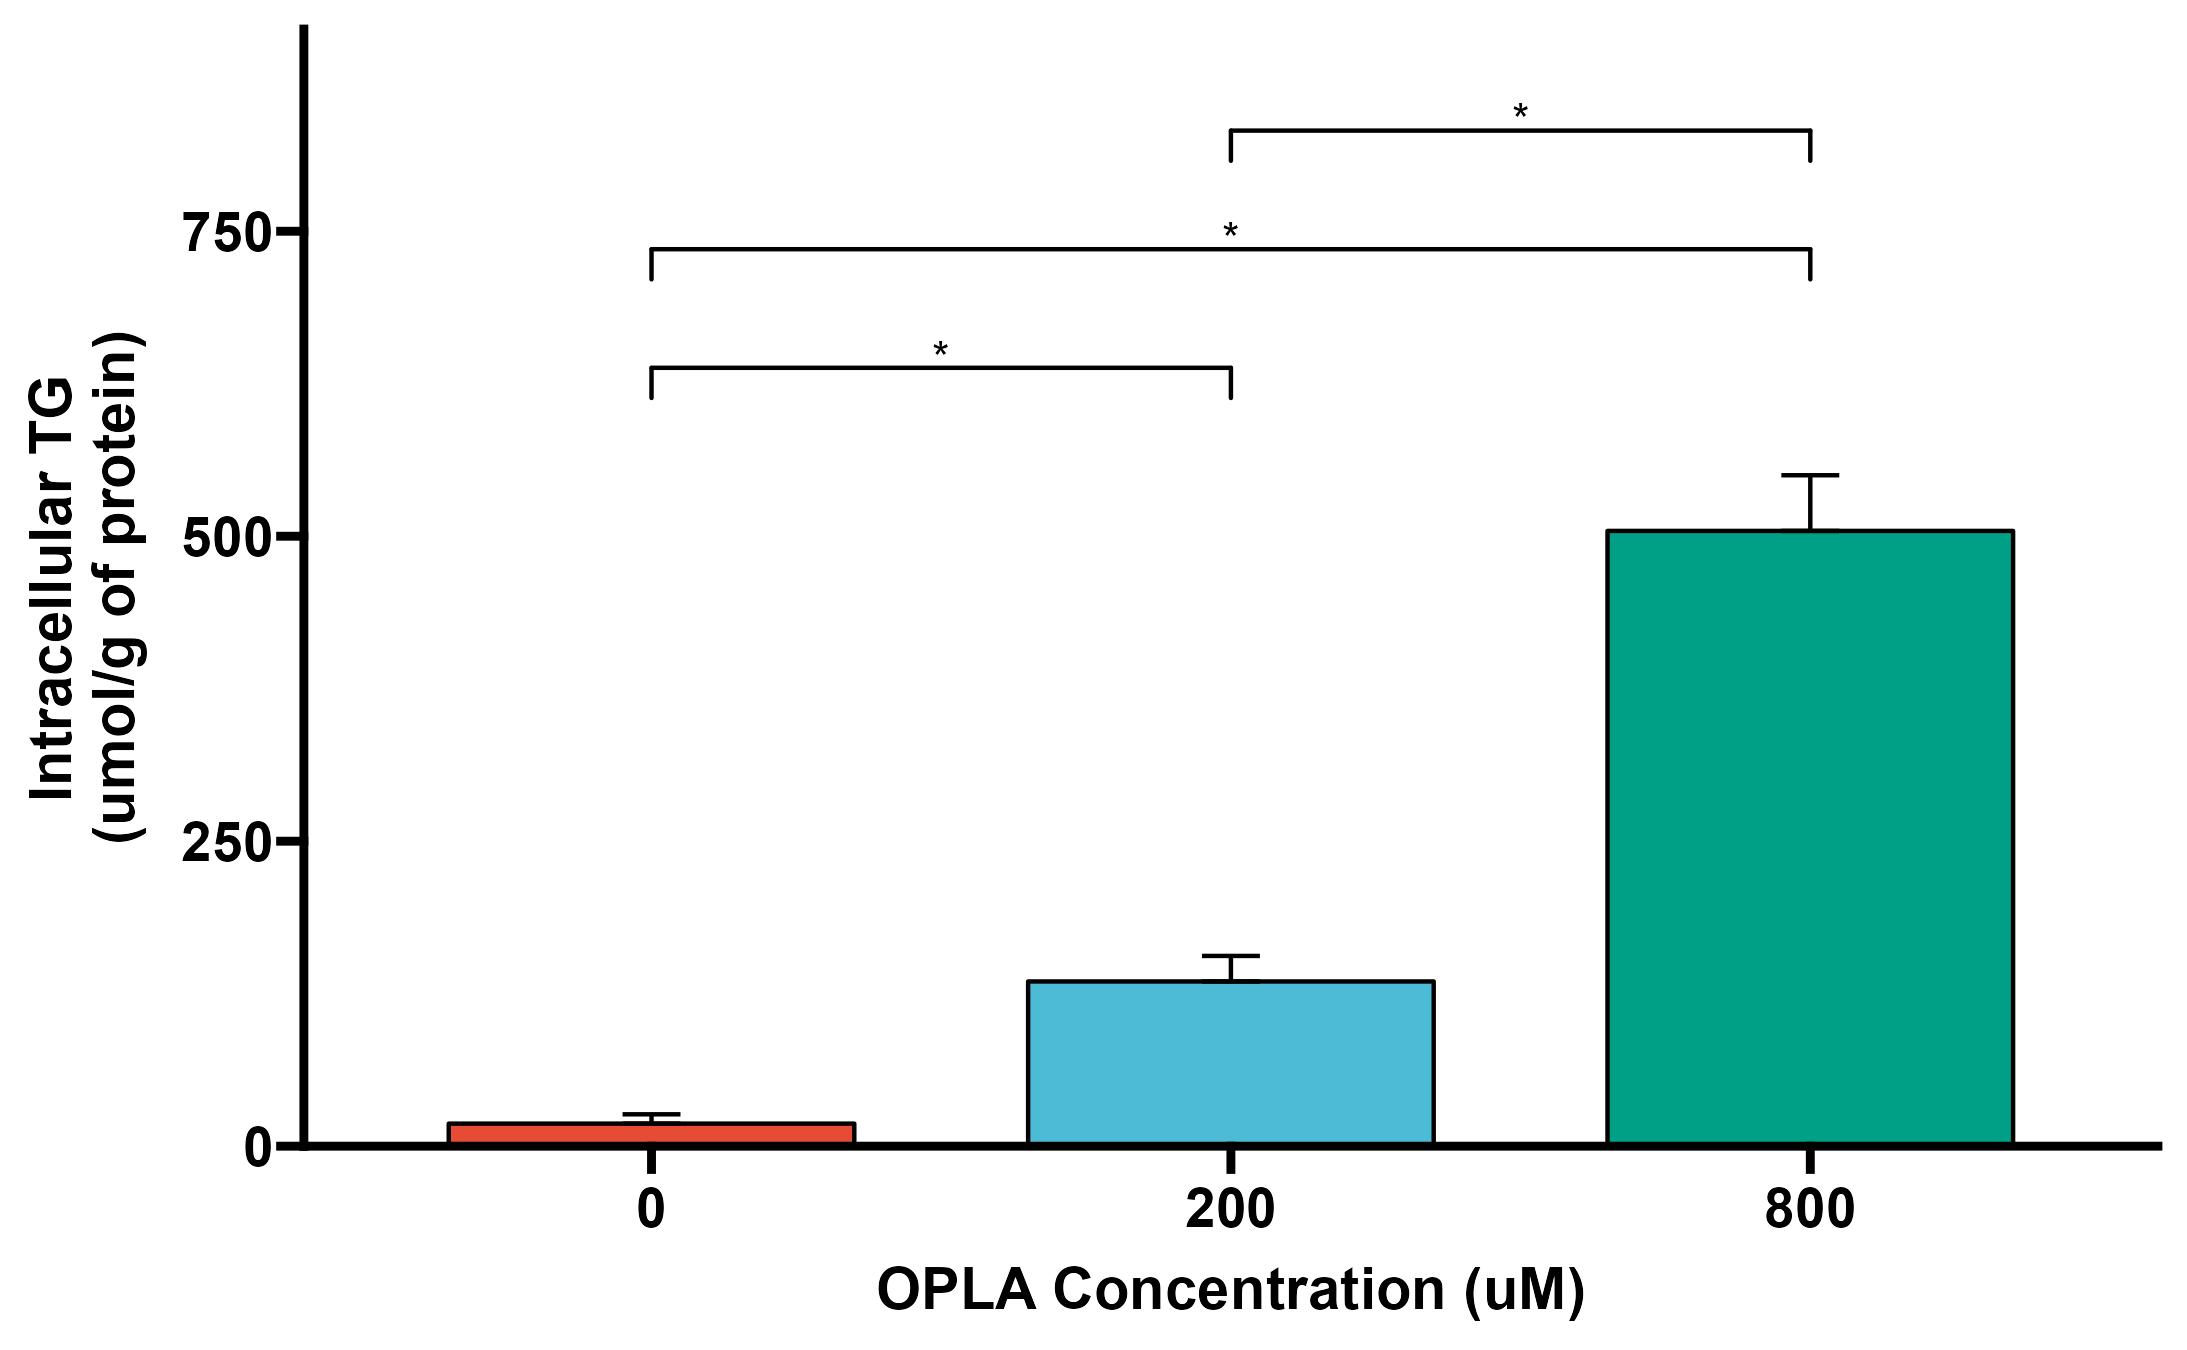
\includegraphics[width=\textwidth]{figures/ch3-Model Development/LFHF TG.png}
     \end{subfigure}  
     \hfill
     \begin{subfigure}[b]{0.49\textwidth}
         \textbf{B}
         \centering
         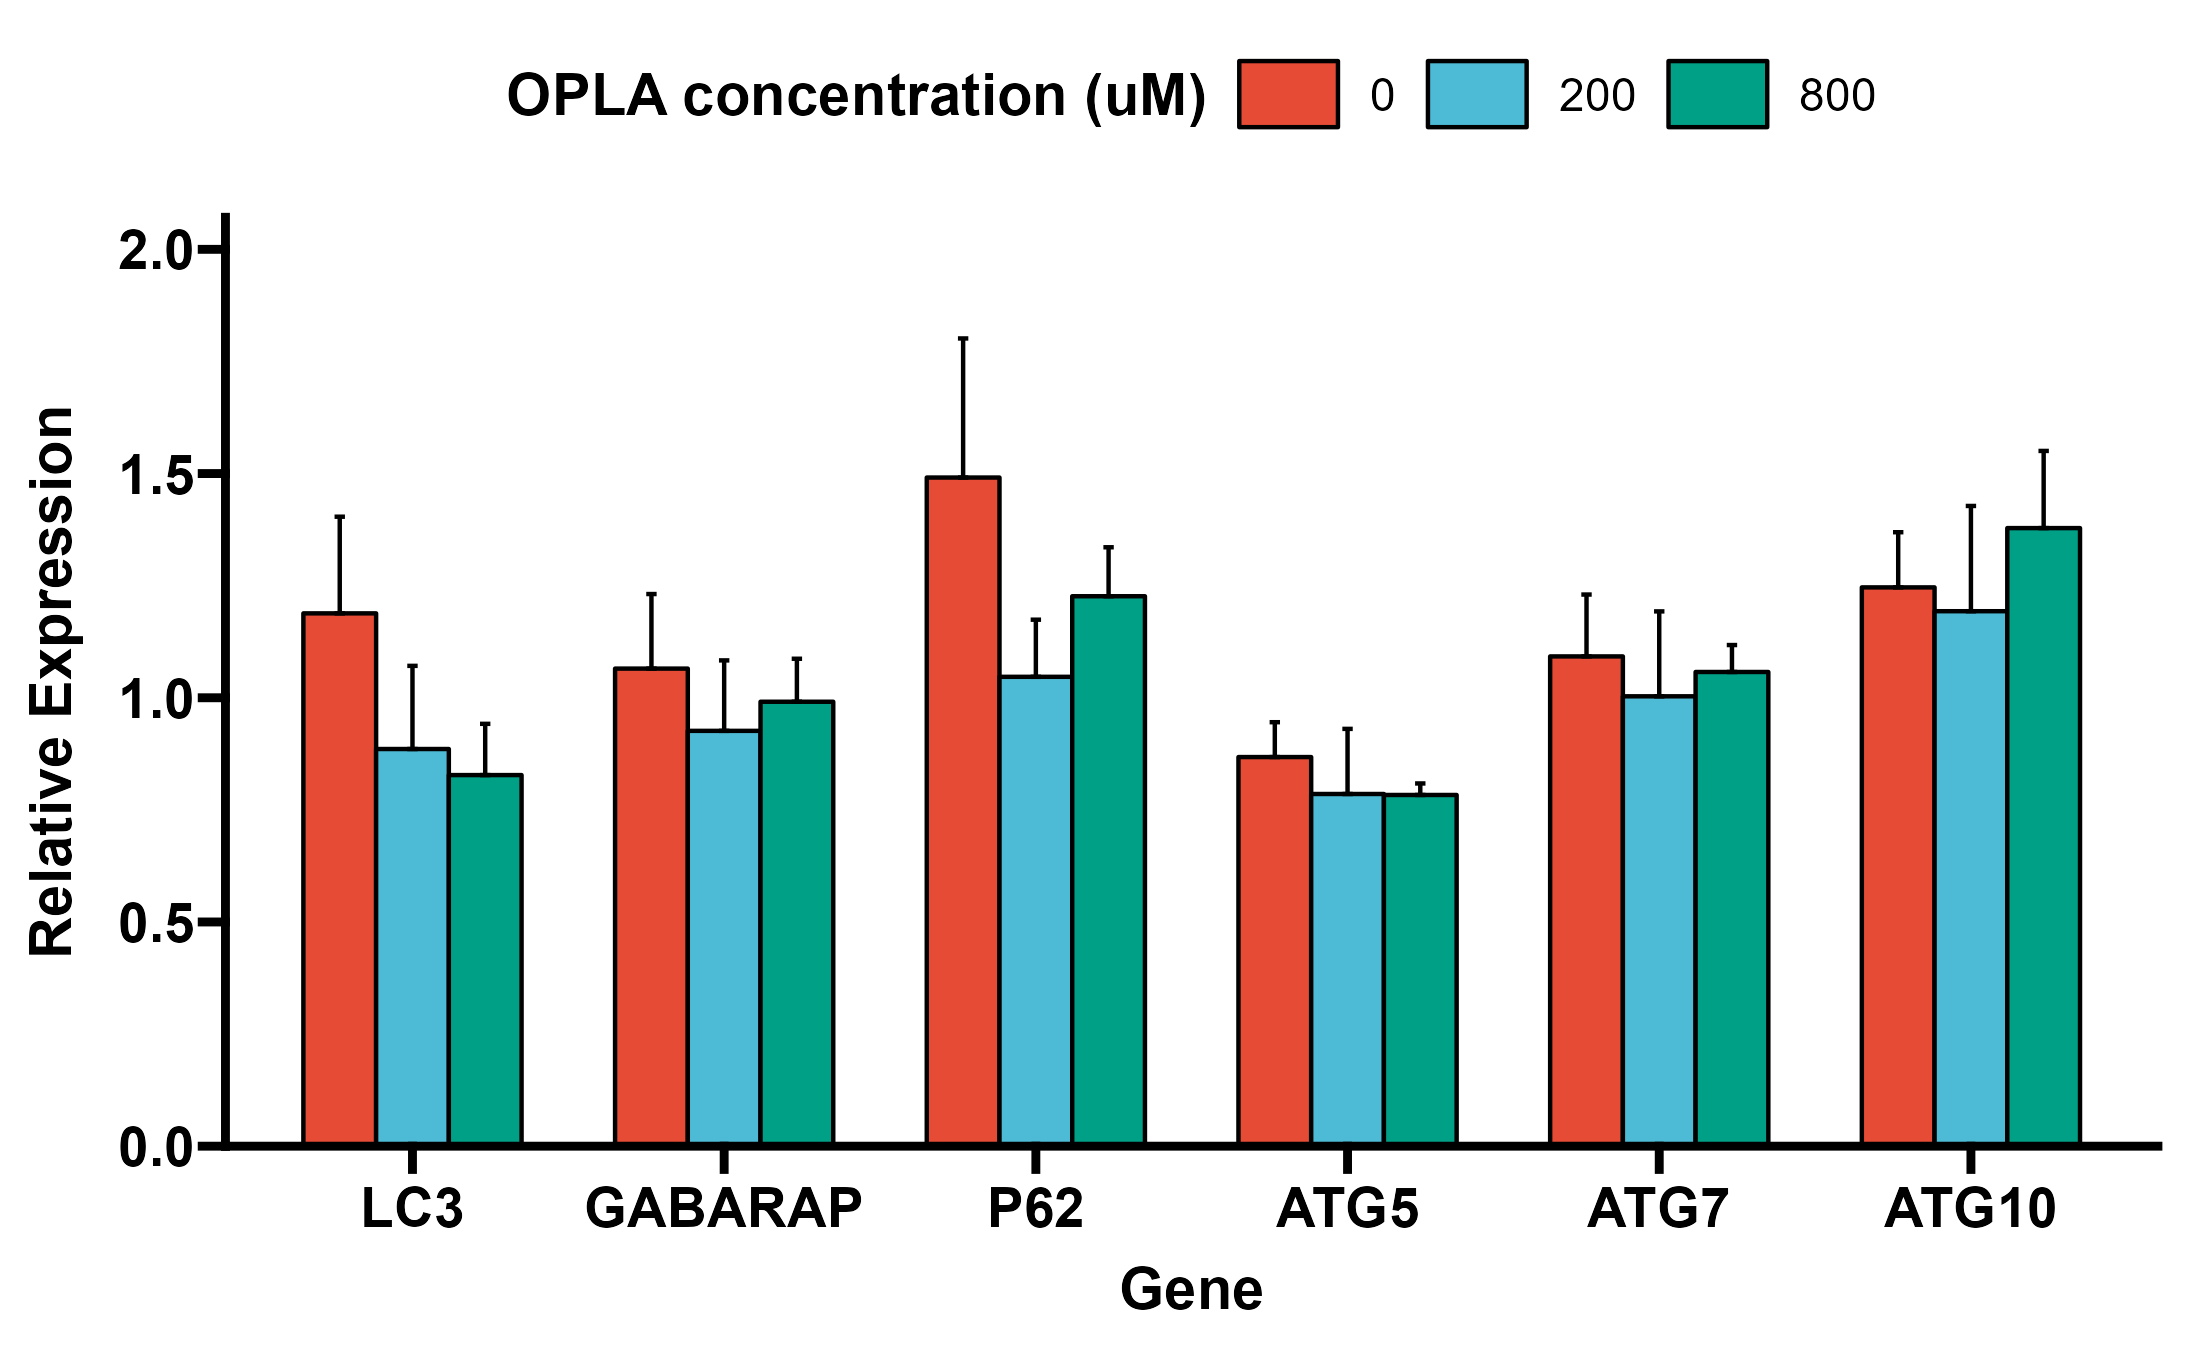
\includegraphics[width=\textwidth]{figures/ch3-Model Development/LFHF ATG genes.png}
     \end{subfigure}
     \hfill
        \caption{\textbf{Effect of media fatty acid concentration on triglyceride accumulation and autophagy.} Huh7 cells were cultured for 7 days in increasing concentrations of OPLA fatty acid mix. \textbf{A)} Lipids were extracted and intracellular triglyceride content quantified by gas chromatography. \textbf{B)} RNA was extracted to measure autophagic gene expression. Representative of three biological repeats (n=3) carried out in technical triplicate. * p < 0.05. Abbreviations: TG, Triglyceride.}
        \label{fig:ch3-Model Development LFHF}
\end{figure}

\subsection{Effect of media FA composition on TG accumulation and autophagy}

Culturing Huh7 cells in predominantly unsaturated (OPLA) or saturated (POLA) FAs resulted in a similar increase in intracellular TG content, when compared to control media free from FAs (Figure \ref{fig:OPLAPOLA}a). Intracellular TG composition reflected that of the FAs the cells were cultured in (Figure \ref{fig:OPLAPOLA}b). Autophagic flux was then assessed by measuring LC3-II protein intensity (relative to housekeeper protein $\alpha$-Tubulin) with and without the autophagic inhibitor BAF. As LC3-II is normally degraded during autophagy, it's accumulation during autophagic inhibition is reflective of overall autophagic flux \cite{DJ2021Guidelines1}. There was no significant difference in autophagic flux between control, OPLA and POLA conditions, though there was a trend towards a decrease in cells treated with FAs (Figures \ref{fig:OPLAPOLA}c-e)..

\begin{figure}[h!]
     \centering
     \begin{subfigure}[b]{0.49\textwidth}
     \textbf{A}
         \centering
         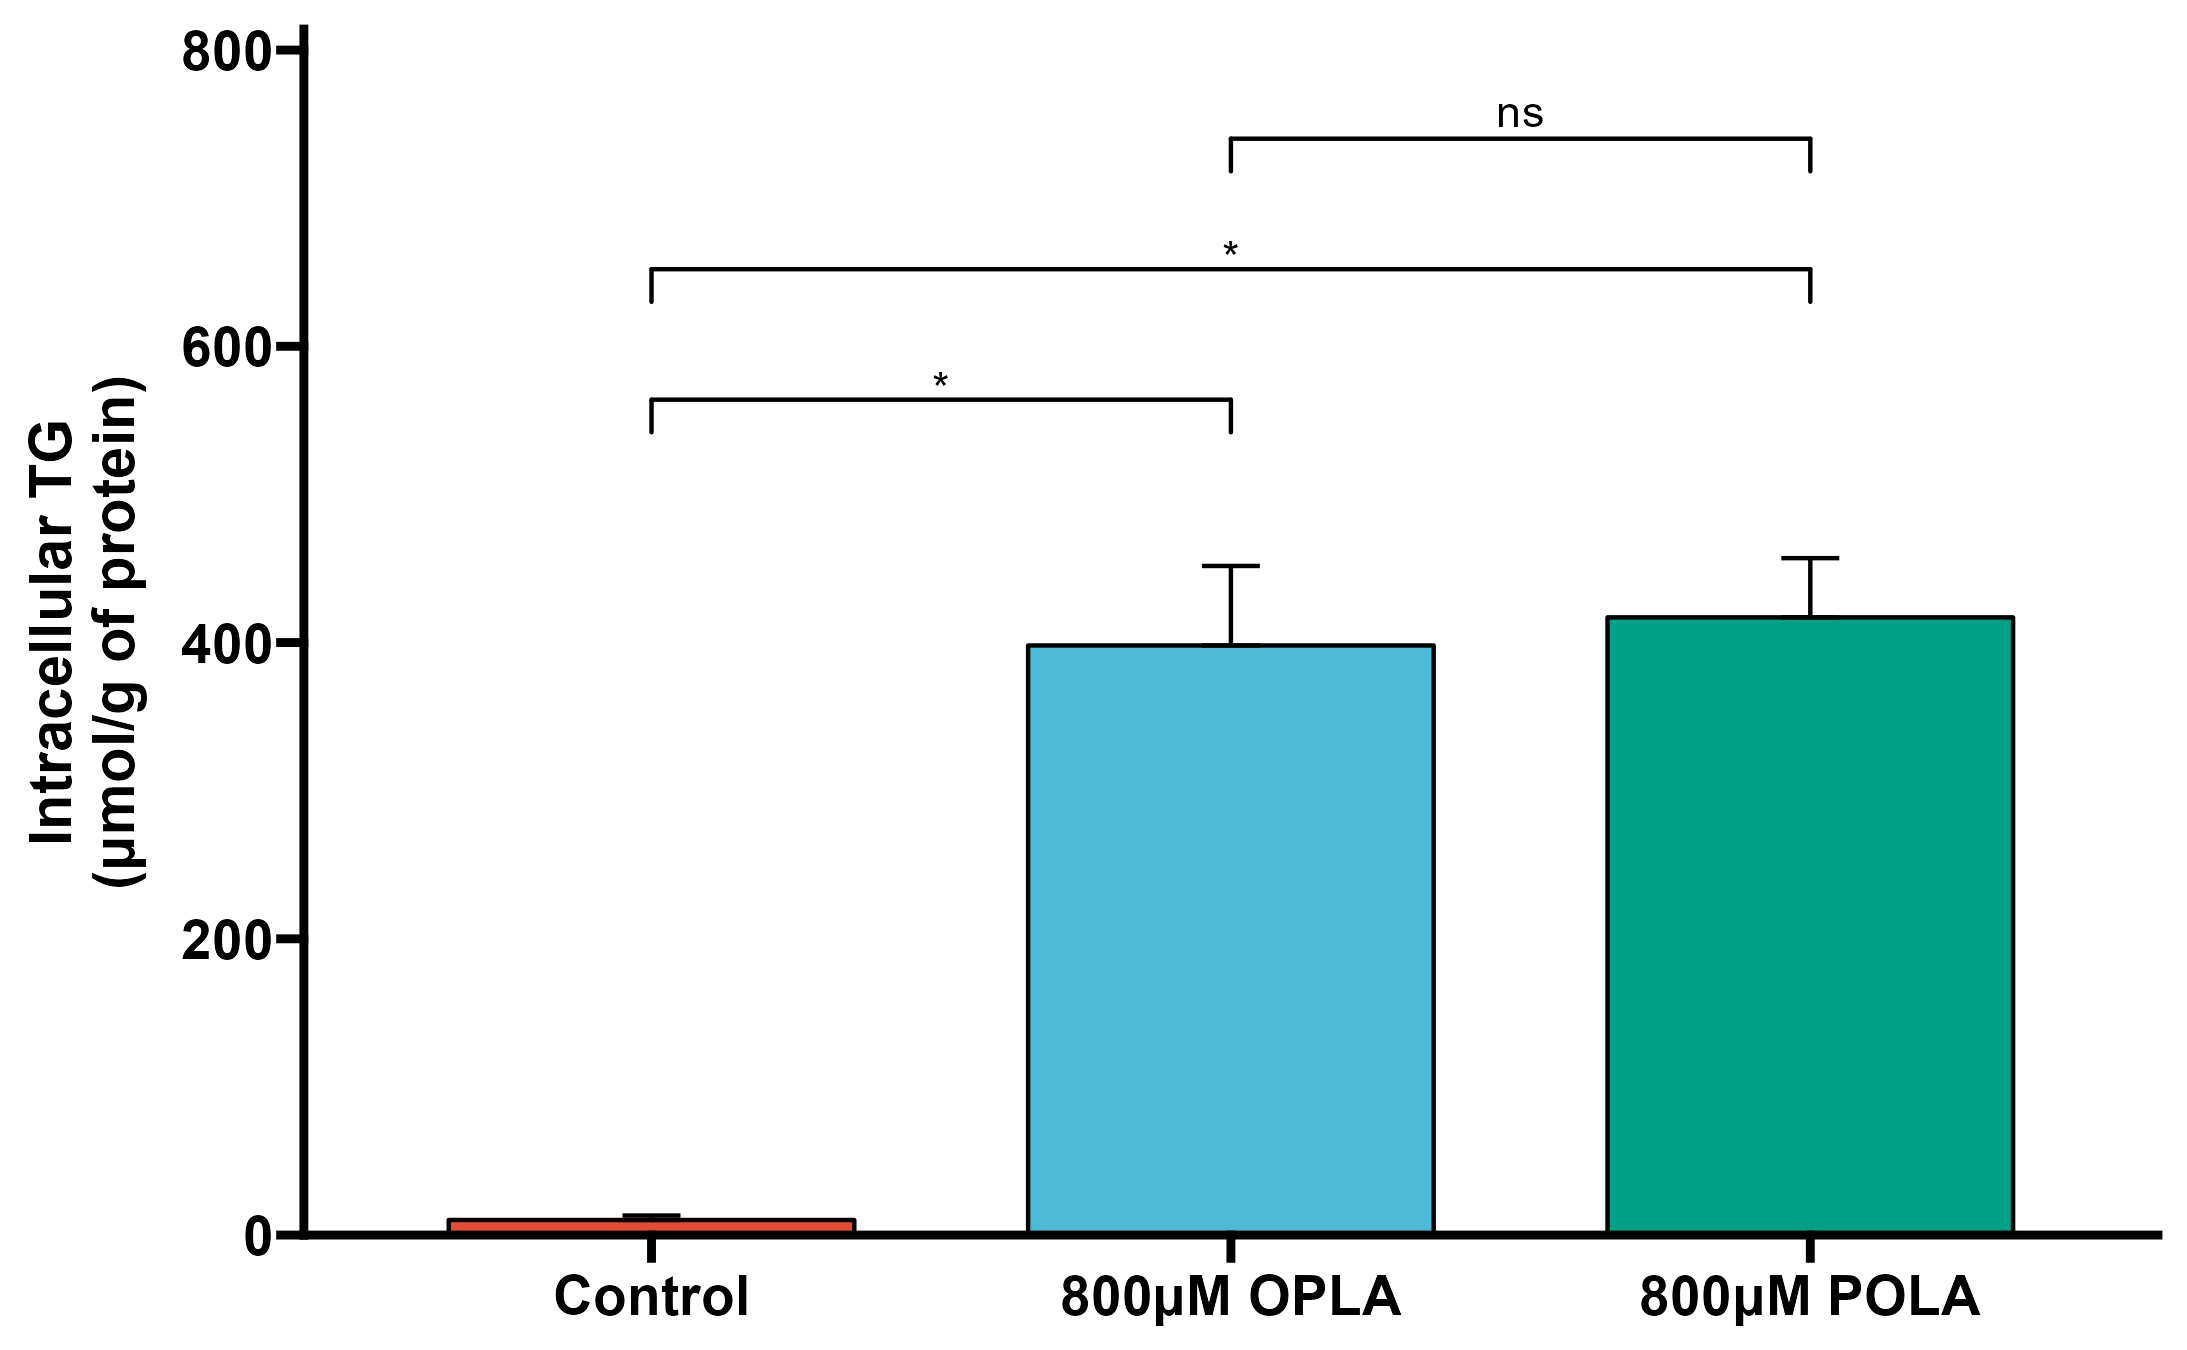
\includegraphics[width=\textwidth]{figures/ch3-Model Development/OPLAPOLA TG.png}
     \end{subfigure}
     \hfill
     \begin{subfigure}[b]{0.49\textwidth}
     \textbf{B}
         \centering
         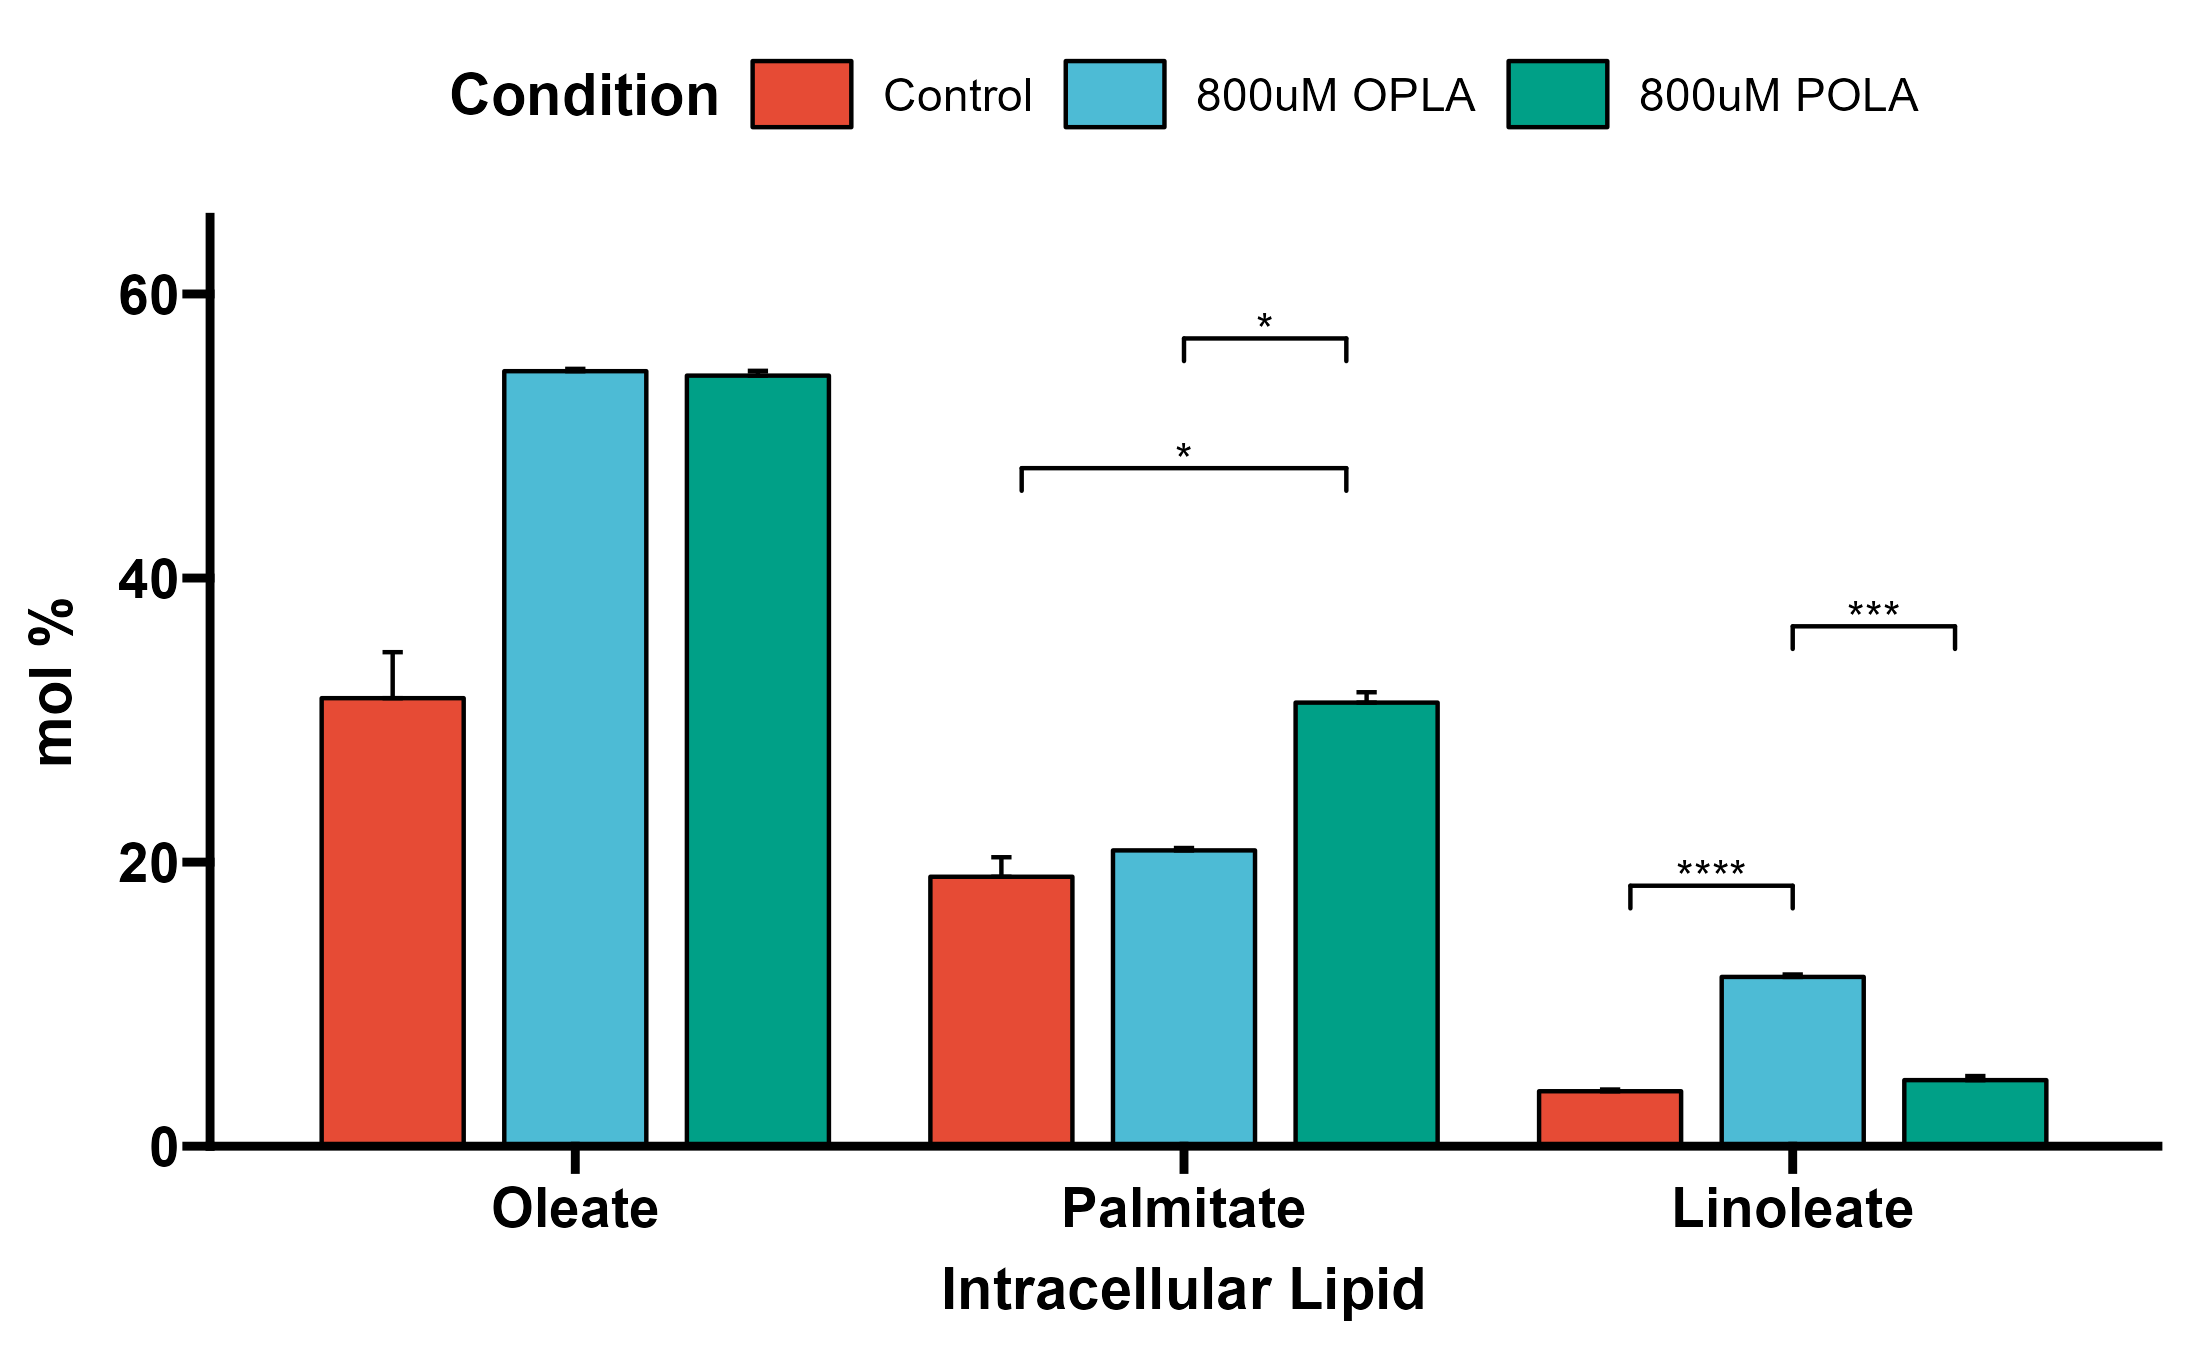
\includegraphics[width=\textwidth]{figures/ch3-Model Development/OPLAPOLA Lipid contributions.png}
     \end{subfigure}
     \hfill
      \begin{subfigure}[b]{0.49\textwidth}
      \textbf{C}
         \centering
         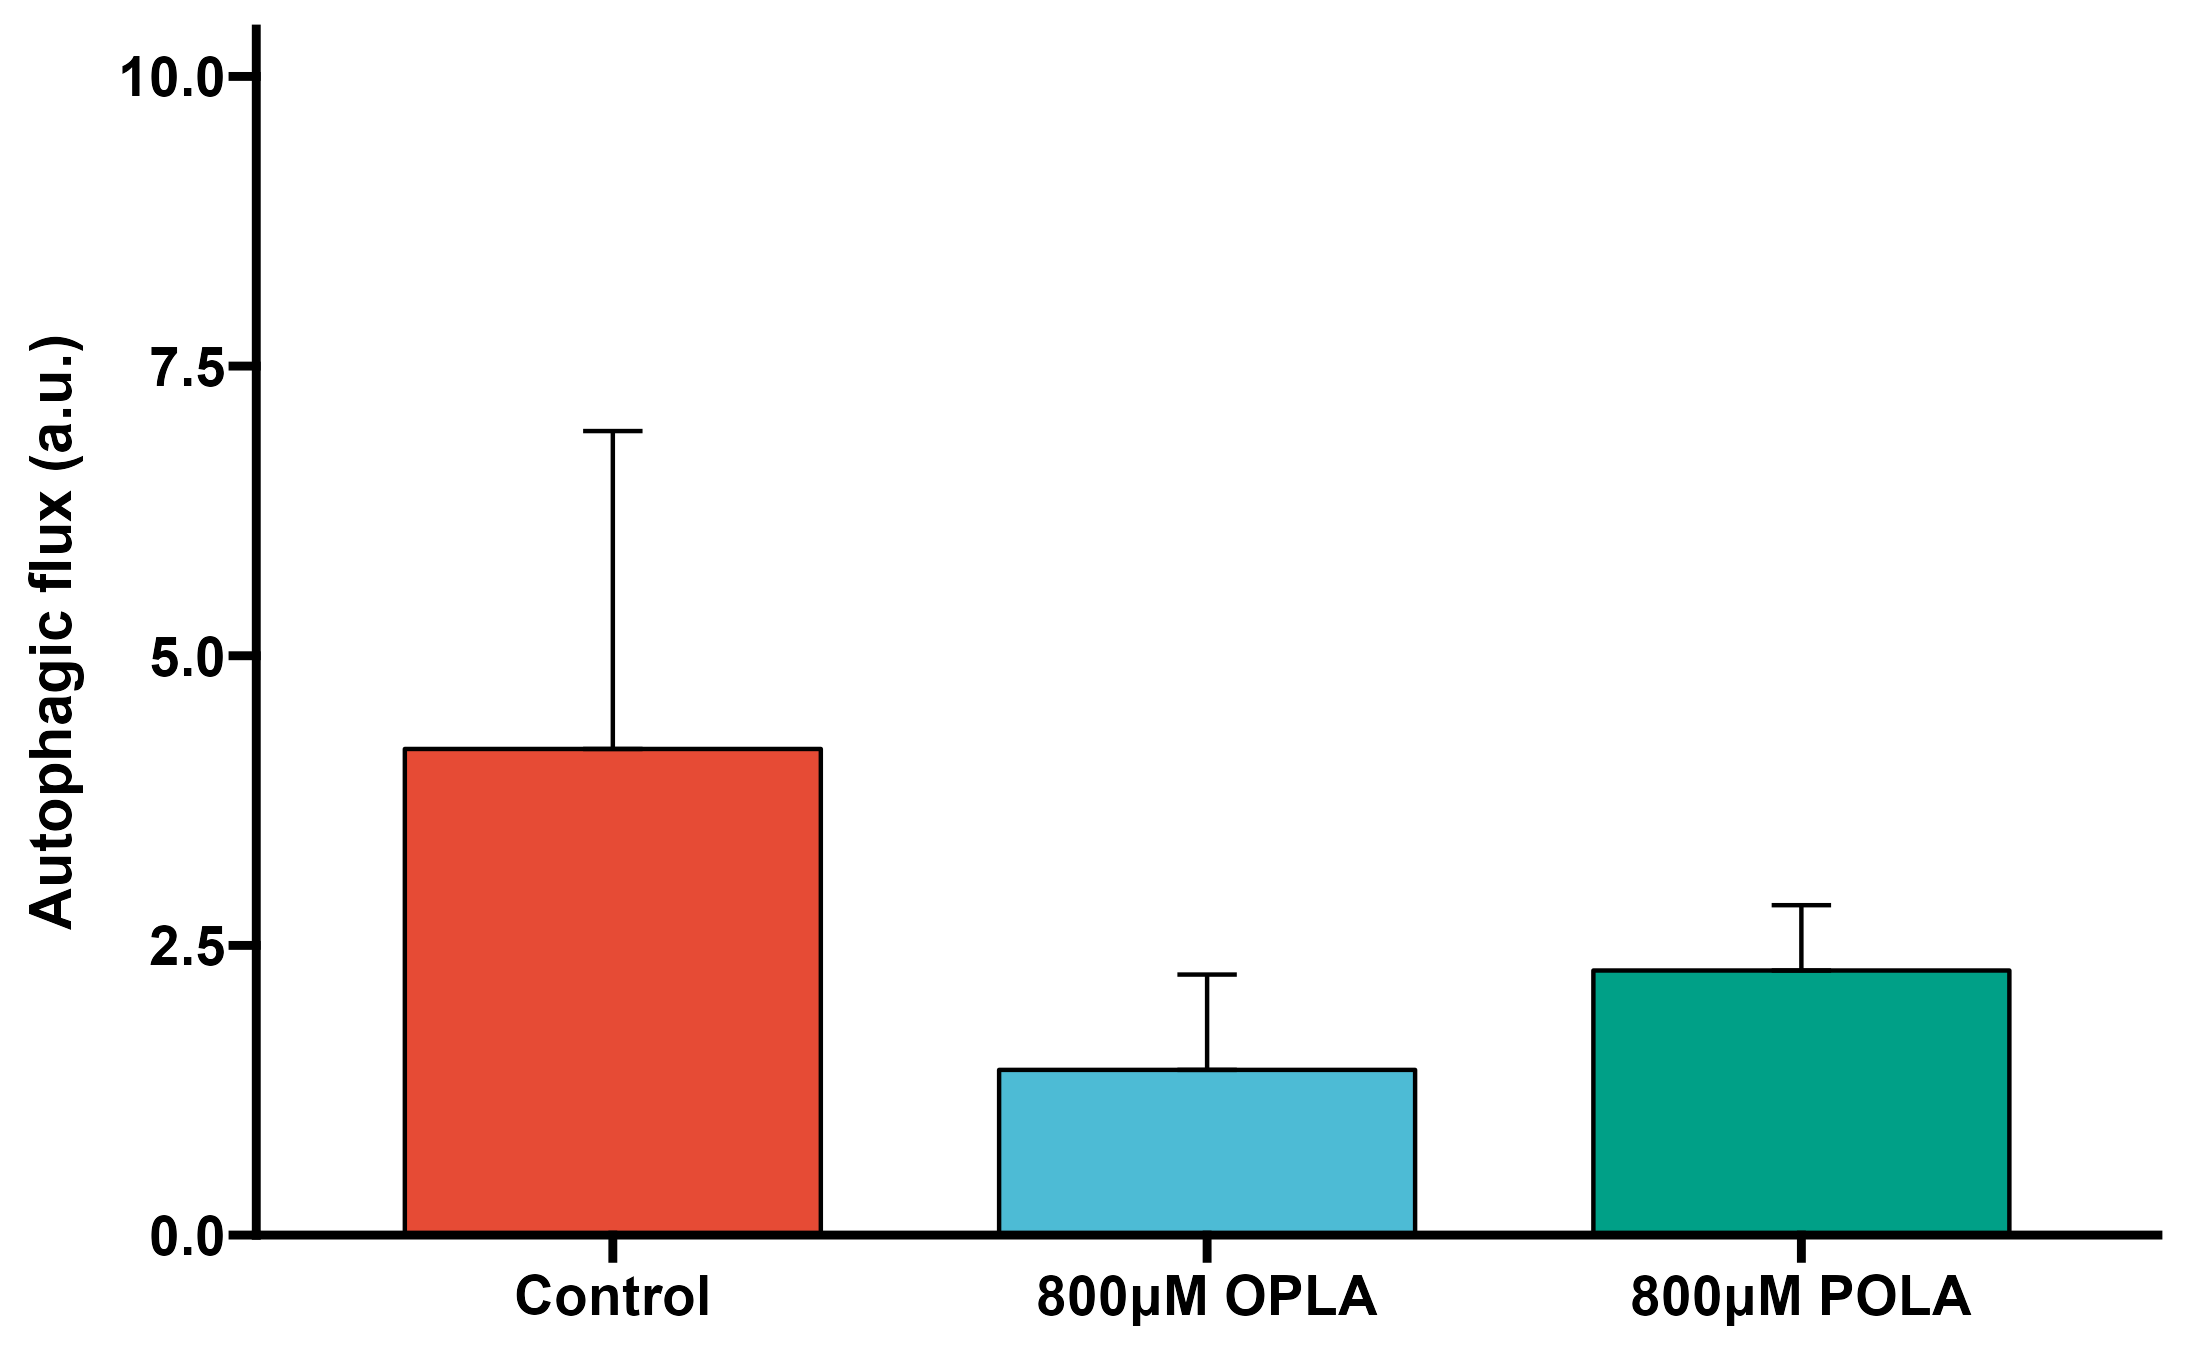
\includegraphics[width=\textwidth]{figures/ch3-Model Development/OPLAPOLA ATG FLX.png}
     \end{subfigure}
     \hfill
       \begin{subfigure}[b]{0.49\textwidth}
       \textbf{D}
         \centering
         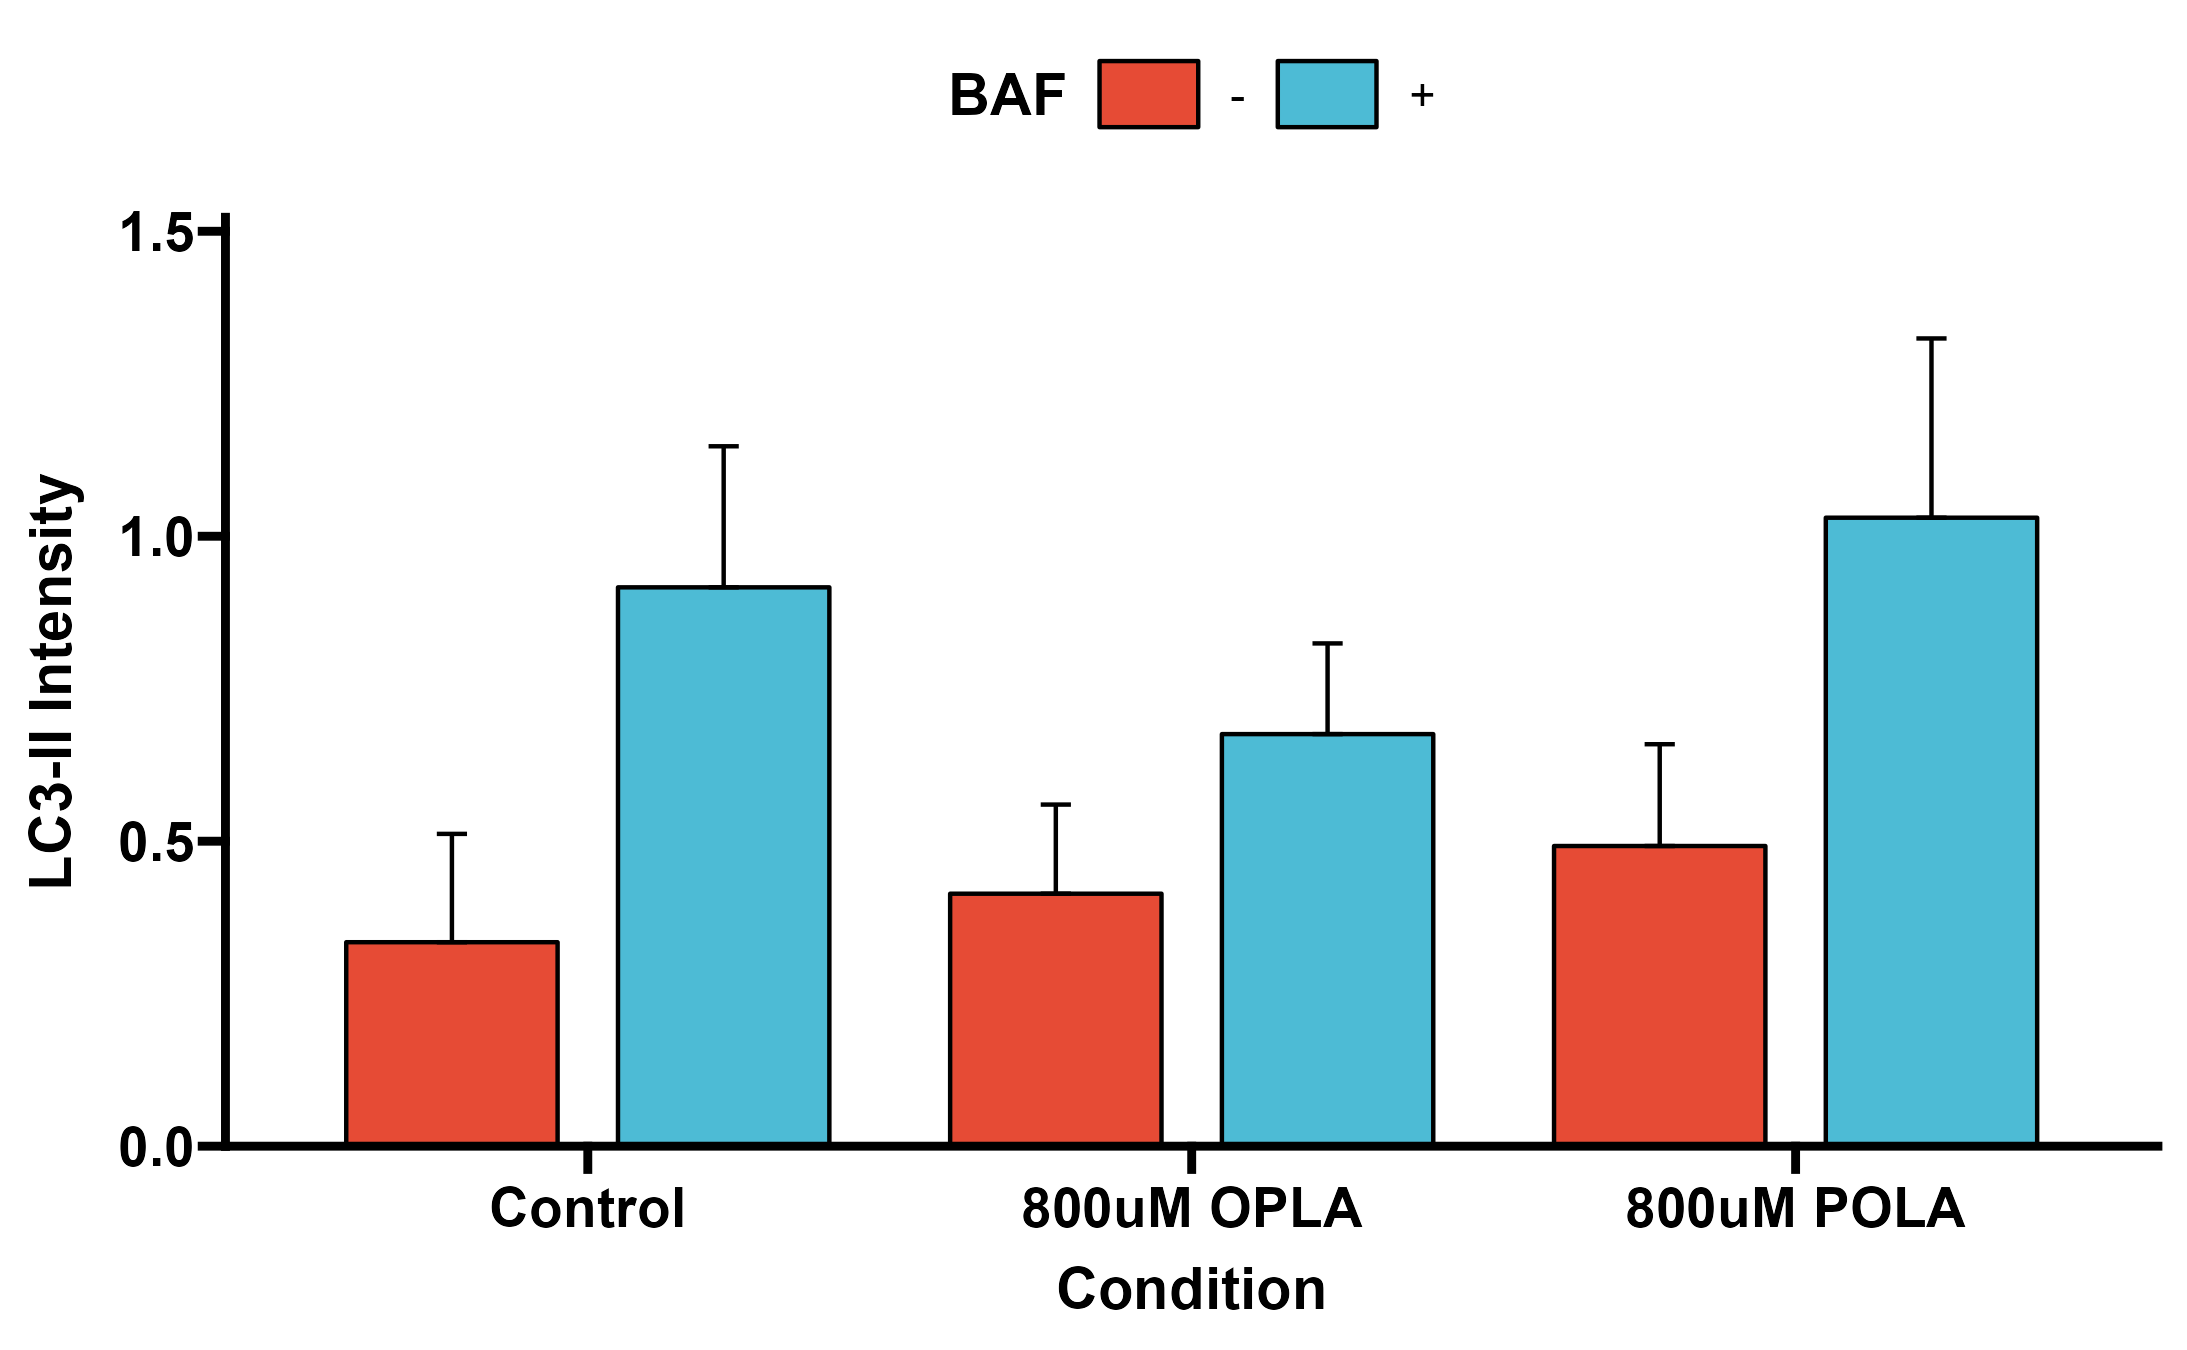
\includegraphics[width=\textwidth]{figures/ch3-Model Development/OPLAPOLA BAF.png}
     \end{subfigure}
     \hfill
       \begin{subfigure}[b]{0.6\textwidth}
       \textbf{E}
         \centering
         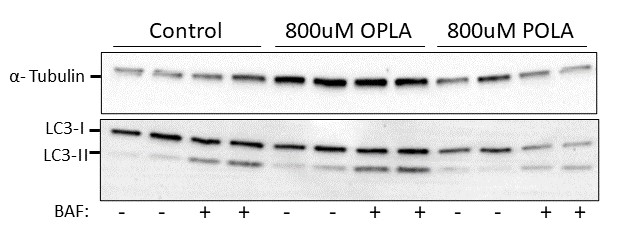
\includegraphics[width=\textwidth]{figures/ch3-Model Development/OPLAPOLA WB Photo.jpg}
     \end{subfigure}
     \hfill
        \caption{Effect of media FA composition on intracellular triglyceride content (a) and composition (b) and autophagic flux (c-e). Autophagic flux calculated as LC3-II intensity (relative to housekeeper protein $\alpha$-Tubulin): (BAF - Basal)/Basal. Representative of three biological repeats (n=3) carried out in technical duplicate. * = p-value < 0.05, ** = p-value < 0.01, *** = p-value < 0.001. Abbreviations: BAF, Bafilomycin A1; TG, Triglyceride.}
        \label{fig:OPLAPOLA}
\end{figure}